% sizes tiny scriptsize footnotesize small normalsize large Large LARGE huge Huge

\documentclass[presentation]{beamer}

\usetheme{JuanLesPins}
\usecolortheme{orchid}
\setbeamertemplate{headline}{}
\setbeamertemplate{navigation symbols}{}

\usepackage{subfig}
\usepackage{listings}
\usepackage{graphicx}
\usepackage[english]{babel}
\usepackage[latin1]{inputenc}
\usepackage{color}
\input{listing_theme.tex}

\usepackage{tikz}


% Add any additional packages you use in your presentation
% -----pack
% \usepackage{xxx}


% -----

% Add your custom definitions etc., if required
% -----misc
% \newcommand{\xxx}[1]{[#1]}
\usetikzlibrary{shapes.geometric, arrows}
\tikzstyle{node} = [rectangle, rounded corners, minimum width=10cm, minimum height=1cm,text centered, draw=black, fill=blue!30]
\tikzstyle{arrow} = [thick,->,>=stealth]
% -----




\title{Optimizations for function calls}
\author[]{Anna Bryta?czyk \and Jakub Sroka}
\institute[]{Akademia G�rniczo-Hutnicza}
\date{16.06.2020}


\begin{document}

\begin{frame}
  \titlepage
\end{frame}

\frame{\tableofcontents}
%%%%%%%%%%%%%%%%%%%%%%%%%%%%%%%%%%%%%%%%%%%%%%%%%%%%%%%%%%%%%%%%%%%
\section{Introduction}
\begin{frame}
	\frametitle{Introduction} 
   Through the code generation process it is possible to obtain some optimizations. The main goal is to make generated code:
   \begin{itemize}
   	\item completely correct
   	\item high speed
   	\item small size
   	\item low energy consumption
   \end{itemize} 
	In presented order if only application doesn't dictate any special requirements.
\end{frame}

\begin{frame}
	\frametitle{Introduction} 
	One of the most efficient techniques of optimisations is to optimize function calls.
	
\end{frame}


%%%%%%%%%%%%%%%%%%%%%%%%%%%%%%%%%%%%%%%%%%%%%%%%%%%%%%%%%%%%%%%%%%%
\section{In-lining}
\begin{frame}[fragile]
	\frametitle{In-lining}
	To clearly explain the idea of in-lining, let's look for the following example in C language:
	
	\begin{columns}
		\begin{column}{0.48\textwidth}
			\begin{lstlisting}[linewidth=\textwidth, basicstyle=\tiny]
void f(){
    ...
    g(numb++);
    ...
}

void g(int i){
    printf("sqrt= %d", i*i);
}
			\end{lstlisting}
		\end{column}
		\begin{column}{0.04\textwidth}
		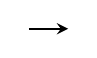
\begin{tikzpicture}
		\tikzstyle{arrow} = [thick,->,>=stealth]
		\draw [arrow](0,0) -- (0.5, 0);
		\end{tikzpicture}
		\end{column}
		\begin{column}{0.48\textwidth}  %%<--- here
					\begin{lstlisting}[linewidth=\textwidth, basicstyle=\tiny]
void f(){
    ...
    {int i=numb++; printf("sqrt= %d", i*i);}
    ...
}

void g(int n){
    printf("Lucky number is: %d", n);
}
					\end{lstlisting}
		\end{column}
	\end{columns}
	
\end{frame}

\begin{frame}
	\textbf{What happened?} \newline
	Mainly, call of function g in AST of f was replaced by the AST of g, but also during in-lining there is a need to handle returned value and parameter transfer. The last two depends on language and here the variable trasfer looks like "int i=variable;". \newline
	Note that in this case naive replacing "i" by "numb++" would be incorrect and that is why "i" declaration is necessary. 
\end{frame}

\begin{frame}
	\frametitle{Why in-lining}
	In-lining eliminate function call with could be expensive, but the real gain of it is "breaking unbreakable barrier of function" as is going on other kinds of optimization.
	\newline\newline
	However, in-lining is recommeded expecially for short functions. In-lining frequently occuring, long functions could cause incresing genreated code size and time of compilation what in some cases is unacceptable.
	\newline\newline
	
	
\end{frame}

\begin{frame}
	\frametitle{Example 2}
	Refering to function g in previous example, let's look what could be done after in-lining of g(4):
	\newline
	\newline
	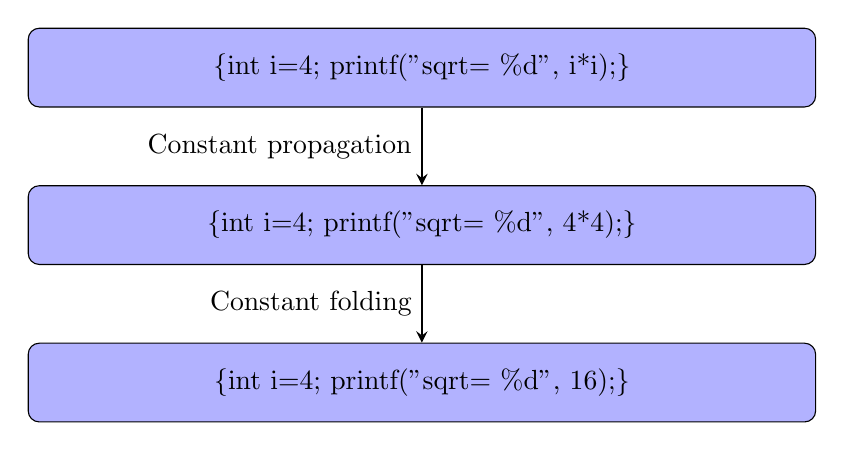
\begin{tikzpicture}[node distance=2cm]
	\node (n1) [node] {\{int i=4; printf("sqrt= \%d", i*i);\}};
	\node (n2) [node, below of=n1] {\{int i=4; printf("sqrt= \%d", 4*4);\}};
	\node (n3) [node, below of=n2] {\{int i=4; printf("sqrt= \%d", 16);\}};

	\draw [arrow] (n1) -- node[anchor=east] {Constant propagation} (n2);
	\draw [arrow] (n2) -- node[anchor=east] {Constant folding} (n3);
	\end{tikzpicture}
	\newline
	\newline
	And now variable "i" is no longer needed, what improves speed. 
\end{frame}
%%%%%%%%%%%%%%%%%%%%%%%%%%%%%%%%%%%%%%%%%%%%%%%%%%%%%%%%%%%%%%%%%%%
\section{Cloning}
\begin{frame}
	\frametitle{Cloning}
	Clonning is similiar idea to in-linning - it also make a copy of function's AST, but in this case not to replace its call but rather to make a new one with at least one parameter replaced by constant. 
\end{frame}

\begin{frame}[fragile]
	\frametitle{Example}
	Consider function "count\_in\_inteval" which returns number of elements from interval [begin, end] that ocuurs in given array.
	\begin{lstlisting}[linewidth=\textwidth, basicstyle=\tiny]
int count_in_inteval(double[] array, int lenght, double begin, double end){
	int couter = 0;
	for(int i=0; i < length; i++)
		if(array[i] >= begin && array[i] <= end) counter++;
	return counter;
}
	\end{lstlisting}
	Call count\_in\_interval(array, lenght, 1.0, 5.0) could at compile time cause preparing cloned function looks like that:
	\begin{lstlisting}[linewidth=\textwidth, basicstyle=\tiny]
int count_in_inteval_1_5(double[] array, int lenght){
	int couter = 0;
	for(int i=0; i < length; i++)
		if(array[i] >= 1.0 && array[i] <= 5.0) counter++;	
	return counter;
}
	\end{lstlisting}
\end{frame}

\begin{frame}
	Note that the arguments begin and end was replaced by constants, so as it is in in-lining here also some optimisation around function block could be done. However, even without additional actions, code become more efective.
	\newline\newline
	A large proportion of the calls with constant parameters concerns calls to library
	routines, and cloning is most effective when the complete program is being optimized,
	including the library routines.
\end{frame}

\end{document}
